\chapter{基于分布式文件系统GlusterFS的数据迁移研究}

\section{GlusterFS介绍}

GlusterFS\cite{GlusterFS}是一个开源、扩展能力强大的分布式文件系统,其客户端与存储服务器可通过InfiniBand RDMA或者TCP/IP等多种方式连接,并使用统一的命名空间管理数据,可将不同类型的存储服务器整合在同一个命名空间中,从而为各种工作负载和应用场景提供出色的性能。 GlusterFS服务器兼容POSIX标准,支持诸如ext4、XFS等{\color{orange}扩展属性文件系统},可以使用包括(Network File System)和SMB(Server Message BLock)等在内的业界标准访问协议进行访问。GlusterFS专为当前高性能虚拟化云环境而设计,也可用于在并行文件系统之上搭建大规模科学与工程计算文件系统。 

本节将对GlusterFS的架构与原理作简要介绍,并重点分析其数据迁移模块Tiering。
\subsection{整体架构和原理}
%\begin{itemize}
%    \item 全局命名空间。
%    \item 集群存储管理。
%    \item 模块化的层次机构。
%    \item 内置replication and geo-replication特性。
%    \item 自修复功能。
%    \item 高效负载均衡。
%\end{itemize}
\begin{figure}[htp]
\centering
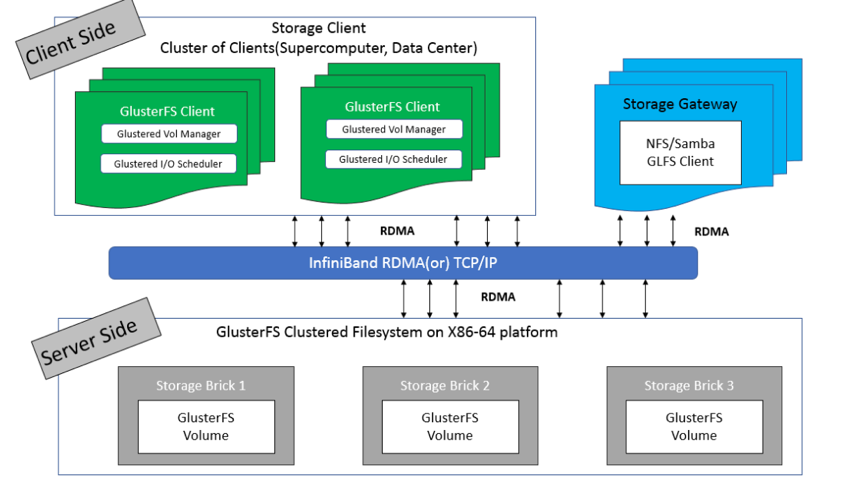
\includegraphics[width=\textwidth]{GlusterFS_Arc}
\caption{GlusterFS整体架构图}
\label{fig:GlusterFS_Arc}
\end{figure}
如图\ref{fig:GlusterFS_Arc}所示,GlusterFS服务端以存储块(Storage Brick)为硬件存储单元,可挂载于磁盘、固态硬盘、内存等多种存储介质。逻辑卷(Volume)是文件系统中的逻辑存储单元,每一个逻辑卷可由一个或者多个存储块构成,绝大多数gluster管理操作是在卷上进行的。GlusterFS根据用户需求能够支持多种逻辑卷,主要包括:

{\color{red}这里itemize的格式有问题}

\begin{itemize}
    \item 分布式卷(Distributed Volume)。文件通过hash算法将数据分布到所有存储服务器上,这种卷是glusterfs的基础和最大特点;其本质功能是扩大的磁盘空间,如果有一个磁盘损坏,其数据也丢失,文件级RAID 0,不具有容错能力。
    \item 复制卷(Replicated Volume)。此类逻辑卷将文件同步复制到多个brick上,文件级RAID 1,具有容错能力,同等硬件条件下写性能下降,但读性能有所提升。
    \item 条带卷(Stripe Volume)。类似RAID0,文件分成数据块以Round Robin方式分布到存储服务器上,并发粒度是数据块,支持超大文件,大文件的读写性能优异。
    \item 复合卷。所谓复合卷主要包括分布式条带卷、分布式复制卷、条带复制卷和分布式条带复制卷等,兼具了基本卷的优点,在实际应用场景下较常见。
\end{itemize}
\begin{figure}[htp]
\centering
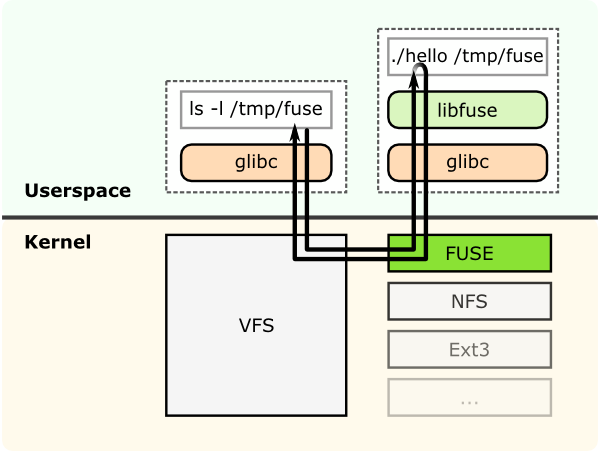
\includegraphics[width=\textwidth]{fuse}
\caption{用户空间文件系统FUSE}
\label{fig:fuse}
\end{figure}
GlusterFS是一个用户空间文件系统,采用了FUSE(File System in Userspace){\color{red}(此处应有引用)}作为用户态程序与内核文件系统交互的接口。如图\ref{fig:fuse}所示,

\subsection{层叠式模块设计}
\begin{figure}[htp]
\centering
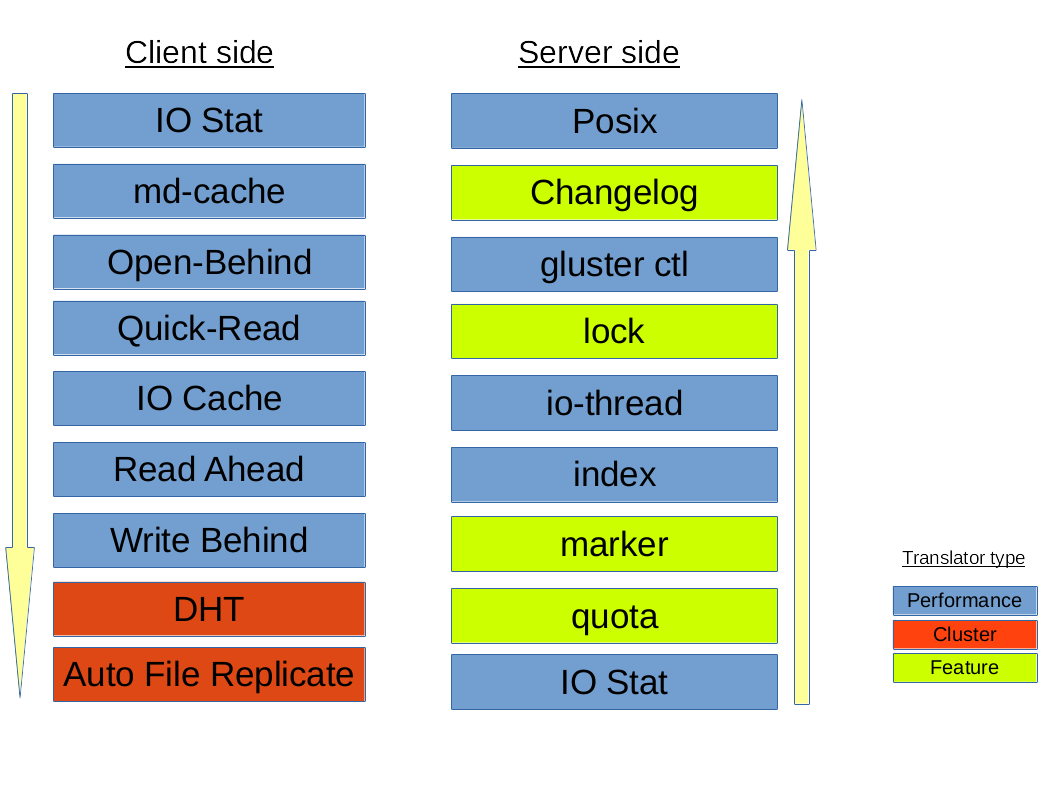
\includegraphics[width=\textwidth]{translators}
\caption{由模块(Translators)堆叠组成的堆栈式结构}
\label{fig:translators}
\end{figure}
Translator是GlusterFS中处理文件请求,实现各类文件操作功能的模块
\cite{BWFS}\cite{DPFS}。
如图\ref{fig:translators}所示,不同功能的模块以动态链接库的方式加载,以函数调用的形式逐级传递和处理文件操作请求,并通过回调函数传回文件操作结果或读取的数据。客户端和服务端之间的消息传递则通过远程过程调用(Remote Procedure Call)实现。
Translator模块是GlusterFS实现诸多功能的主要组件,每一层translator模块内均可对POSIX文件操作函数(打开文件、读写数据和元数据访问等)重新定义,可通过修改参数或修改回调数据等方式实现特定功能。Translator模块以一对一或一对多的方式堆叠组合实现更复杂的功能。

%GlusterFS主要包括cluster,performance,features,protocal,storage,encryption等几类模块。其中cluster类模块是实现存储集群功能的核心,包括分布式哈希表(DHT),
GlusterFS主要包括以下几组translator模块:
\begin{enumerate}
    \item 集群模块组(Cluster Translators)。主要包括分布式哈希表(DHT)、自动文件备份(AFR)等模块,是构成存储服务器集群功能的核心组件。GlusterFS没有采用元数据服务器定位文件数据,而是采用弹性哈希算法定位文件,首先根据文件路径计算哈希值,然后根据哈希值定位到具体的brick存储单元进行文件定位。AFR模块的功能则是自动冗余备份(为避免分歧,通常备份数据多于两个),当发生数据丢失或损坏时进行数据修复。
    \item 性能模块组(Performance Translators)。此类模块的目的是对GlusterFS的整体性能进行优化,如io-cache在GlusterFS进程的内存池内空闲部分开辟空间用于缓存;io-threads用于多线程管理;md-cache用于元数据缓存服务;read-ahead用于预读数据;write-back实现写回功能提升写数据性能等等。
    \item 功能模块组(Feature Translators)。主要包括日志管理模块changelog,全局锁管理locks模块等等。
    \item 协议模块组(Protocol Translators)。GlusterFS架构下,客户端与存储服务端互联方式多种多样,通过协议模块组实现对多种标准协议的支持。
    \item 存储模块组(Storage Translators)。实现GlusterFS与本地POSIX文件系统的接口。
    \item 加密模块组(Encryption Translators)。顾名思义,可以在此类模块中灵活定义不同的加密算法以保证数据安全性。
    \item 调试模块组(Debug Translators)。
\end{enumerate}

\subsection{Tiering模块}
\begin{figure}[htp]
\centering
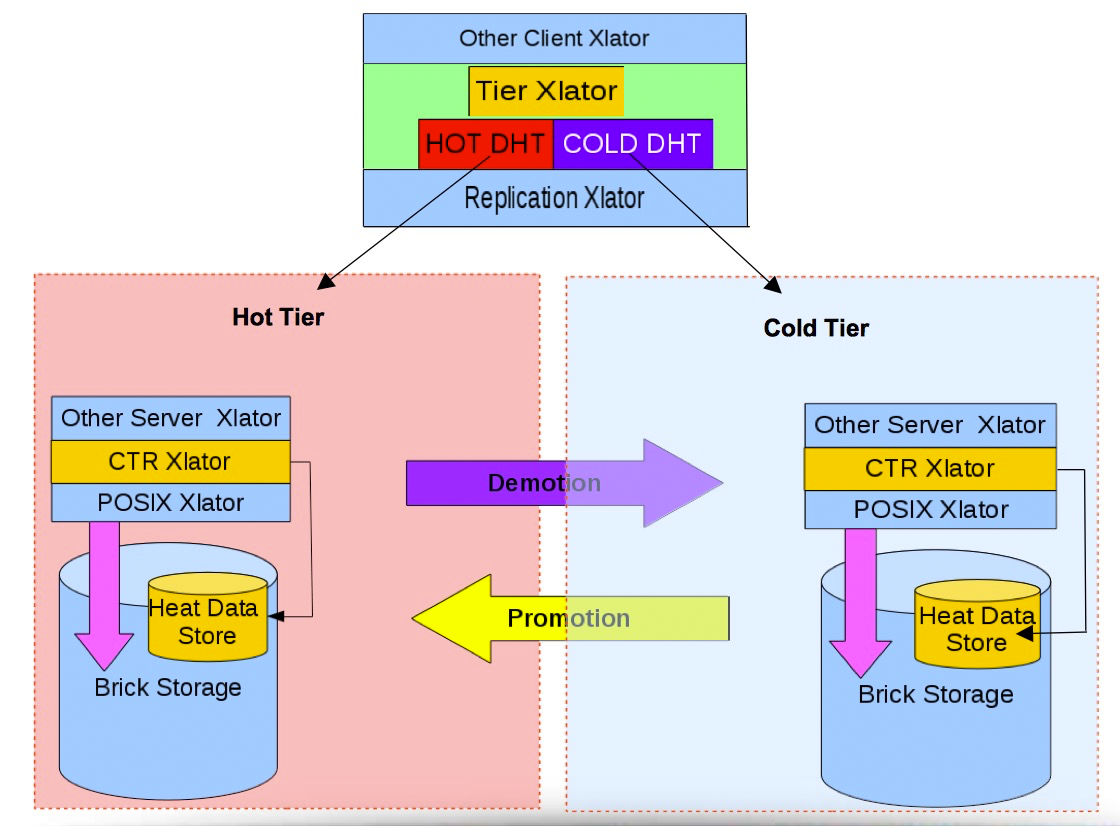
\includegraphics[width=\textwidth]{tiering}
\caption{Tiering模块原理}
\label{fig:tiering}
\end{figure}
Tiering模块是GlusterFS自3.7之后开始支持的分层数据管理模块\cite{Tiering}。与传统分层存储思想类似,文件数据被冠以“热”与“冷”的分类标签,即,访问频繁的文件为“热”数据,反之为“冷”数据。在Tiering模块的实现中,同一逻辑卷被同时挂载到“冷热”两类brick存储单元,“热”存储单元(通常为高性能存储介质如DRAM或SSD等)被视为“冷”存储(廉价、性能较弱的磁盘)的上一级缓存,因此文件的“冷热”对用户应用透明,完全由tiring模块负责文件分类与缓存调度。

如图\ref{fig:tiering},当GlusterFS启用tiering模块时,原本的分布式哈希算法模块被调整为“热”哈希模块与“冷”哈希模块。文件定位与查找优先在“热”存储内进行,若查找成功就是一次缓存命中;反之发生缓存缺失时通过“冷”哈希模块将请求转发到“冷”存储进行重新定位查找。

传统缓存替换算法LRU的实现过程中的核心指标是数据近期访问次数(通常存储于访问速度最快的L1-cache中),近期最少访问的数据被淘汰,而tiering模块则沿用了这一思想。区别在于tiering模块中缓存置换的粒度远远大于CPU cache或内存级的缓存,大多数应用场景是将SSD作为磁盘阵列的缓存,需要迁移置换的数据量大(大文件或海量小文件),同时算法的时间粒度也要宽松得多。

基于上述原因,GlusterFS基于sqlite3实现了一个专门用于记录文件访问记录的数据库libgfdb。该数据库用于记录存储单元内所有已知文件的元数据,作为文件“冷热”分类的依据。

\begin{table}[htbp]
\centering
\begin{minipage}[t]{0.9\linewidth}
\caption{Libgfdb中的元数据结构}
\label{tab:libgfdb_file}
\begin{tabularx}{\linewidth}{cZ}
\toprule[1.5pt]
{\hei 元数据} & 描述\\
\midrule[1pt]
GF\_ID & 文件的GFID\\
W\_SEC, W\_MSEC & 写操作请求发起(wind)时间,以秒或毫秒为单位\\
UW\_SEC, UW\_MSEC & 写操作{\color{red}返回}时间\\
U\_READ\_SEC, W\_READ\_MSEC & 读操作请求发起时间\\
UW\_READ\_SEC, W\_READ\_MSEC & 读操作{\color{red}返回}时间\\
WRITE\_FREQ\_CNTR & 写操作频率\\
READ\_FREQ\_CNTR & 读操作频率\\
\bottomrule[1.5pt]
\end{tabularx}
\end{minipage}
\end{table}

\begin{table}[htbp]
\centering
\begin{minipage}[t]{0.9\linewidth}
\caption{Libgfdb目录入口表(Directory Entries)}
\label{tab:libgfdb_flink}
\begin{tabularx}{\linewidth}{cZ}
\toprule[1.5pt]
元数据 & 描述\\
\midrule[1pt]
GF\_ID & 文件的GFID(复合主键)\\
GF\_PID & 父目录的GFID(复合主键)\\
FNAME & 文件名(复合主键)\\
FPATH & 完整路径\\
W\_DEL\_FLAG & 文件删除(unlinked)标志\\
LINK\_UPDATE & 文件重命名标志\\
\bottomrule[1.5pt]
\end{tabularx}
\end{minipage}
\end{table}

表\ref{tab:libgfdb_file}记录了所有已知文件的访问情况,包括文件操作的起始时间,访问频率等。表\ref{tab:libgfdb_flink}本质上是libgfdb维护的目录入口表,主要用于文件查找。

除“冷热”哈希模块外,另一个关键模块是访问计数器模块CTR(Change Time Recorder)。该模块位于底层POSIX模块之上,其主要功能是对存储单元内所有文件的访问情况进行记录,包括近期内数据读、数据写和元数据写等操作的执行次数等,用于更新libgfdb数据库。

当一个逻辑卷启用tiering模块时,将会在后台开启数据迁移进程。该进程周期性地查询数据库,以获得最近的文件访问情况,从而完成{\color{orange}迁入}(promotion)与{\color{orange}迁出}的数据迁移操作。

在系统运行过程中,数据迁移决策同样受到”热“存储占用率的影响。默认设置下,当“热”存储占用未达到75\%时,即便没有达到周期性迁移的时间节点,系统也会自动将“冷”存储单元内的高频率访问文件迁入“热”存储单元,以防止迁出过多数据导致缓存空间的浪费;当“热”存储占用超过默认的90\%时,将自动地触发迁出操作,以防止到达缓存容量上限降低整体性能。

\section{基于Tiering模块的主动预取框架设计}
如上节所述,GlusterFS实现的tiering模块主要采用传统的LRU算法设计,能够显著改善大文件的连续读操作,但对于一些不具备“缓存友好”性质的工作负载,例如多客户端并发访问大量小文件的场景下,tiering的性能提升不够明显
\cite{Red_Hat_Gluster_storage_on_supermicro_storage_servers_powered_by_Intel_Xeon_processors}。

其本质原因是随着小文件数量大幅增加,且多客户端的并发文件请求数量上升时,传统缓存置换算法考虑的时间局部性和空间局部性失去效用,仅仅简单地以文件访问频率作为考量不足以分析提取复杂场景下的I/O访问模式。


\subsection{Trace 模块}
\subsection{访问模式识别模型建立}
\subsection{运行时缓存管理}


\section{本章小结}